\chapter{Un lecteur virtuel de codes-barres}

Après que l'application de test ait été achevée, je me retrouvai sans activité alors qu'il me restait la moitié de mon stage.
C'est ainsi que je me lançai dans un projet de détecteur virtuel de codes-barres.
Me basant sur le moteur de détection de GdPicture que je connaissais désormais, j'ai développé une application ergonomique et simple qui simule un lecteur de codes-barres sur des images ou des documents scannés.

\section{Objectifs}

Cette application devait tout d'abord reproduire le fonctionnement des lecteurs de codes-barres filaires existants.
Il devait être possible d'accéder rapidement à l'application depuis n'importe quelle autre, et que le lecteur soit une extension de la souris.
Enfin, plusieurs actions devaient être possibles une fois un code-barres détecté :
\begin{itemize}
\item Copier le résultat dans le presse-papier
\item Envoyer le résultat vers une autre fenêtre pour qu'elle le traite comme une entrée clavier
\end{itemize}

\section{Développement}

J'ai choisi de créer une application sans fenêtre, c'est à dire qui s'exécuterait d'une manière transparente pour l'utilisateur, et accessible depuis la zone de notifications\footnote{En anglais : \og system tray \fg{} ou plus simplement \og systray \fg{}}.
J'ai pour cela utilisé une bibliothèque WPF\footnote{Disponible ici : http://www.hardcodet.net/projects/wpf-notifyicon} prenant en charge cette fonctionnalité. Il m'est alors possible de créer une icône dans le systray, de créer un menu pour le clic-droit, de gérer les événements de clic et les info-bulles.

On peut voir dans la figure \ref{systrayMenu} le menu de l'application :
\begin{itemize}
\item Une case à cocher pour copier automatiquement le résultat d'une détection dans le presse-papiers
\item Una case à cocher pour l'envoyer dans une fenêtre.
\item Une liste pour choisir ladite fenêtre
\item Un bouton \og Plus d'options \fg{} qui ouvre une fenêtre permettant de choisir les types de codes-barres que l'on souhaite détecter.
\end{itemize}

\begin{figure}
\begin{center}
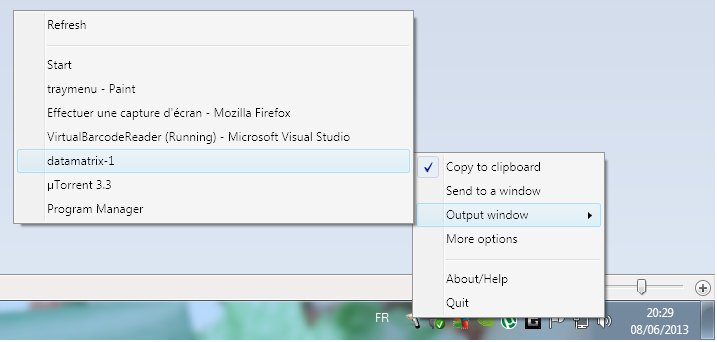
\includegraphics[scale=0.7]{images/traymenu.png}
\end{center}
\caption{Le lecteur de code-barres dans le systray}
\label{systrayMenu}
\end{figure}


\section{Bilan}